\section{Results}
\label{sec:results}

\subsection{Reproducing published results}
\label{sec:res-repro}

\begin{table}[t]
\centering
\caption{Reproduction of published School results. Explained variance (EV, within schools, \%; higher is better) under the protocol of \citet{argyriou2008convex} ($\rho = 75\%$) and RMSE in exam points (lower is better) under the protocol of \citet{kumar2012learning} ($\rho = 60\%$). Ours: mean $\pm$ s.d.\ over 10 random splits. Published values are copied from the cited papers; blank cells were not reported or not run. The bottom four rows are published methods we did not re-implement.}
\label{tab:repro}
\small
\setlength{\tabcolsep}{2.7pt}
\begin{tabular}{@{}llccccc@{}}
\toprule
& & \multicolumn{3}{c}{EV within schools (\%), $\rho = 75\%$} & \multicolumn{2}{c}{RMSE, $\rho = 60\%$} \\
\cmidrule(lr){3-5}\cmidrule(l){6-7}
Method & Published counterpart & Ours & A08 & ZY10 & Ours & KD12 \\
\midrule
Pooled ridge & Aggregate & $22.0 \pm 1.6$ & $22.7 \pm 1.3$ &  & $10.34 \pm 0.06$ &  \\
Independent ridge & Independent / STL & $22.1 \pm 1.8$ & $23.8 \pm 2.1$ & $23.5 \pm 1.9$ & $10.34 \pm 0.05$ & $10.67 \pm 0.20$ \\
$\ell_{2,1}$ MTL & MTL-FEAT (var.\ sel.) & $23.6 \pm 1.8$ & $24.8 \pm 2.0$ &  & $10.27 \pm 0.06$ &  \\
Trace-norm MTL & MTL-FEAT / MTFL & $26.5 \pm 1.5$ & $26.7 \pm 2.0$ & $26.7 \pm 2.0$ & $10.07 \pm 0.06$ &  \\
Mean-reg.\ MTL &  & $27.3 \pm 1.5$ &  &  & $10.02 \pm 0.06$ &  \\
Mean + low-rank MTL &  & $27.3 \pm 1.5$ &  &  & $10.02 \pm 0.06$ &  \\
\midrule
Multi-task GP & MTGP & & & $29.2 \pm 1.6$ & & \\
MTRL & MTRL & & & $29.9 \pm 1.8$ & & \\
No-group MTL & No-group MTL & & & & & $10.18 \pm 0.15$ \\
GO-MTL & GO-MTL & & & & & $10.04 \pm 0.24$ \\
\bottomrule
\end{tabular}

\vspace{2pt}
{\footnotesize A08: \citet{argyriou2008convex}; ZY10: \citet{zhang2010convex}; KD12: \citet{kumar2012learning}.}
\end{table}


\Cref{tab:repro} compares our implementation with three published sets of School results. Under the protocol of \citet{argyriou2008convex}, all four methods with a published counterpart land within one standard deviation of the reported value, and trace-norm MTL is within 0.2 points (26.5\% against 26.7\%). The ranking is identical: pooled and independent ridge are close, $\ell_{2,1}$ MTL is slightly better, and trace-norm MTL is clearly better, winning on all 10 splits against independent ridge by $4.4 \pm 0.5$ points. Under the protocol of \citet{kumar2012learning}, trace-norm MTL reaches an RMSE of 10.07 exam points against 10.04 reported for GO-MTL, another method that ties tasks to a shared low-dimensional basis. Our independent ridge baseline (10.34) is stronger than the published one (10.67), which used a different feature encoding (26 attributes) and tuning procedure. The two partial-pooling estimators score 27.3\% explained variance and 10.02 RMSE, above every linear method we reproduced but below the published MTRL and multi-task Gaussian process results, which we did not re-implement.

\subsection{Learning curves: the pooled model wins when data are scarce}
\label{sec:res-curves}

\begin{figure}[t]
\centering
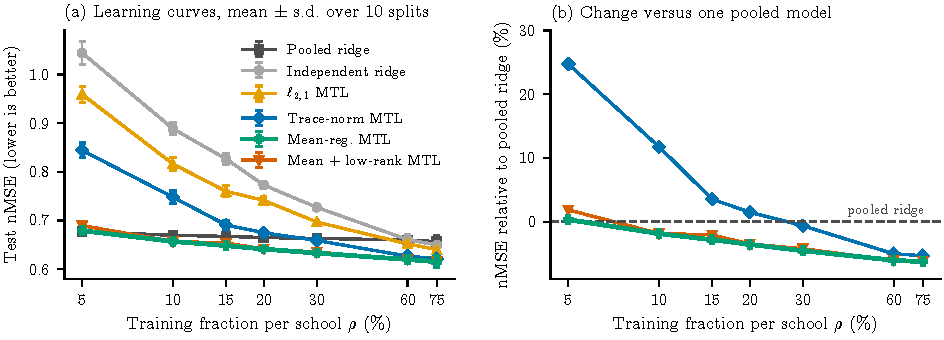
\includegraphics[width=\textwidth]{fig2_learning_curves.pdf}
\caption{Test nMSE as a function of the training fraction per school (log scale). (a) Absolute error; error bars are one standard deviation over 10 splits. (b) Error relative to pooled ridge for the three strongest multi-task methods; negative values beat the pooled model. Trace-norm MTL overtakes pooled ridge only between 20\% and 30\%, whereas mean-regularized MTL (thick green) is at or below the pooled model at every training fraction.}
\label{fig:curves}
\end{figure}

\begin{table}[t]
\centering
\caption{Test nMSE (MSE divided by the variance of test scores; lower is better) as a function of the training fraction per school $\rho$. Mean $\pm$ s.d.\ over 10 random splits; best in bold, second best underlined.}
\label{tab:main}
\small
\setlength{\tabcolsep}{3.6pt}
\begin{tabular}{@{}lccccccc@{}}
\toprule
& \multicolumn{7}{c}{Training fraction per school $\rho$} \\
\cmidrule(l){2-8}
Method & 5\% & 10\% & 15\% & 20\% & 30\% & 60\% & 75\% \\
\midrule
Pooled ridge & \textbf{.677}\,{\scriptsize$\pm$.004} & .669\,{\scriptsize$\pm$.003} & .667\,{\scriptsize$\pm$.001} & .665\,{\scriptsize$\pm$.002} & .663\,{\scriptsize$\pm$.004} & .660\,{\scriptsize$\pm$.008} & .656\,{\scriptsize$\pm$.013} \\
Independent ridge & 1.045\,{\scriptsize$\pm$.023} & .889\,{\scriptsize$\pm$.012} & .826\,{\scriptsize$\pm$.012} & .773\,{\scriptsize$\pm$.006} & .727\,{\scriptsize$\pm$.004} & .660\,{\scriptsize$\pm$.009} & .649\,{\scriptsize$\pm$.012} \\
\midrule
$\ell_{2,1}$ MTL & .959\,{\scriptsize$\pm$.016} & .816\,{\scriptsize$\pm$.014} & .760\,{\scriptsize$\pm$.011} & .741\,{\scriptsize$\pm$.007} & .697\,{\scriptsize$\pm$.004} & .652\,{\scriptsize$\pm$.006} & .640\,{\scriptsize$\pm$.012} \\
Trace-norm MTL & .844\,{\scriptsize$\pm$.015} & .748\,{\scriptsize$\pm$.013} & .691\,{\scriptsize$\pm$.010} & .675\,{\scriptsize$\pm$.004} & .659\,{\scriptsize$\pm$.003} & .626\,{\scriptsize$\pm$.007} & .621\,{\scriptsize$\pm$.012} \\
\midrule
Mean-reg.\ MTL & \underline{.679}\,{\scriptsize$\pm$.008} & \textbf{.657}\,{\scriptsize$\pm$.004} & \textbf{.648}\,{\scriptsize$\pm$.002} & \textbf{.641}\,{\scriptsize$\pm$.003} & \textbf{.633}\,{\scriptsize$\pm$.004} & \underline{.620}\,{\scriptsize$\pm$.008} & \textbf{.615}\,{\scriptsize$\pm$.012} \\
Mean + low-rank MTL & .689\,{\scriptsize$\pm$.007} & \underline{.657}\,{\scriptsize$\pm$.003} & \underline{.653}\,{\scriptsize$\pm$.003} & \underline{.641}\,{\scriptsize$\pm$.002} & \underline{.635}\,{\scriptsize$\pm$.004} & \textbf{.619}\,{\scriptsize$\pm$.008} & \underline{.616}\,{\scriptsize$\pm$.013} \\
\bottomrule
\end{tabular}
\end{table}

\begin{table}[t]
\centering
\caption{Paired comparisons on the same splits. Each cell gives the relative nMSE change of the first method against the second (\%, negative means the first method is better) and, in parentheses, the number of the 10 splits on which the first method wins. $^{\dagger}$: two-sided $p < 0.05$ under the corrected resampled $t$-test of \citet{nadeau2003inference}, which is conservative when the test set is much larger than the training set (small $\rho$). Indep.: independent ridge; Pooled: pooled ridge; Trace: trace-norm MTL; MR: mean-regularized MTL; MLR: mean + low-rank MTL.}
\label{tab:paired}
\footnotesize
\setlength{\tabcolsep}{4.2pt}
\begin{tabular}{@{}lccccccc@{}}
\toprule
& \multicolumn{7}{c}{Training fraction per school $\rho$} \\
\cmidrule(l){2-8}
Comparison & 5\% & 10\% & 15\% & 20\% & 30\% & 60\% & 75\% \\
\midrule
Trace vs.\ Indep. & $-19.2$\,{\scriptsize(10)} & $-15.9$$^{\dagger}$\,{\scriptsize(10)} & $-16.4$$^{\dagger}$\,{\scriptsize(10)} & $-12.7$$^{\dagger}$\,{\scriptsize(10)} & $-9.4$$^{\dagger}$\,{\scriptsize(10)} & $-5.2$$^{\dagger}$\,{\scriptsize(10)} & $-4.4$$^{\dagger}$\,{\scriptsize(10)} \\
Trace vs.\ Pooled & $+24.7$$^{\dagger}$\,{\scriptsize(0)} & $+11.7$\,{\scriptsize(0)} & $+3.5$\,{\scriptsize(0)} & $+1.5$\,{\scriptsize(0)} & $-0.7$\,{\scriptsize(8)} & $-5.0$$^{\dagger}$\,{\scriptsize(10)} & $-5.3$$^{\dagger}$\,{\scriptsize(10)} \\
MR vs.\ Pooled & $+0.3$\,{\scriptsize(4)} & $-1.9$\,{\scriptsize(10)} & $-2.8$$^{\dagger}$\,{\scriptsize(10)} & $-3.6$$^{\dagger}$\,{\scriptsize(10)} & $-4.6$$^{\dagger}$\,{\scriptsize(10)} & $-6.1$$^{\dagger}$\,{\scriptsize(10)} & $-6.3$$^{\dagger}$\,{\scriptsize(10)} \\
MR vs.\ Trace & $-19.6$\,{\scriptsize(10)} & $-12.2$\,{\scriptsize(10)} & $-6.1$\,{\scriptsize(10)} & $-5.0$$^{\dagger}$\,{\scriptsize(10)} & $-3.9$$^{\dagger}$\,{\scriptsize(10)} & $-1.1$\,{\scriptsize(9)} & $-1.0$$^{\dagger}$\,{\scriptsize(10)} \\
MLR vs.\ Pooled & $+1.8$\,{\scriptsize(1)} & $-1.9$\,{\scriptsize(10)} & $-2.1$\,{\scriptsize(10)} & $-3.5$$^{\dagger}$\,{\scriptsize(10)} & $-4.3$$^{\dagger}$\,{\scriptsize(10)} & $-6.1$$^{\dagger}$\,{\scriptsize(10)} & $-6.1$$^{\dagger}$\,{\scriptsize(10)} \\
MLR vs.\ Trace & $-18.3$$^{\dagger}$\,{\scriptsize(10)} & $-12.2$$^{\dagger}$\,{\scriptsize(10)} & $-5.4$\,{\scriptsize(10)} & $-4.9$$^{\dagger}$\,{\scriptsize(10)} & $-3.6$$^{\dagger}$\,{\scriptsize(10)} & $-1.1$\,{\scriptsize(10)} & $-0.8$$^{\dagger}$\,{\scriptsize(10)} \\
MLR vs.\ MR & $+1.5$\,{\scriptsize(0)} & $+0.0$\,{\scriptsize(3)} & $+0.8$\,{\scriptsize(1)} & $+0.1$\,{\scriptsize(4)} & $+0.3$\,{\scriptsize(0)} & $-0.0$\,{\scriptsize(4)} & $+0.1$\,{\scriptsize(2)} \\
\bottomrule
\end{tabular}
\end{table}


\Cref{fig:curves} and \cref{tab:main} show how each method behaves as the training fraction grows from 5\% to 75\%. The usual multi-task story holds against independent models: trace-norm MTL beats independent ridge on all 10 splits at every training fraction, by 19.2\% in nMSE at 5\% and 4.4\% at 75\%, and $\ell_{2,1}$ MTL sits between the two (\cref{tab:paired}).

The pooled model tells a different story. Its error barely changes with the amount of data (nMSE 0.677 at 5\% and 0.656 at 75\%), because the part of the scores it cannot explain is school-specific. Yet at small training fractions it beats every per-school method. Trace-norm MTL is worse than pooled ridge on all 10 splits up to 20\% training, by 24.7\% at 5\% and still 1.5\% at 20\%. It overtakes the pooled model between 20\% and 30\% (better on 8 of 10 splits at 30\%) and is clearly better only at 60\% and 75\% (10 of 10 splits, about 5\%). Independent ridge does not beat the pooled model until 75\%.

\subsection{Why the pooled model wins}
\label{sec:res-why}

Two properties combine. The first is in the data. Seven columns, including the bias, are constant within every school (\cref{sec:setup}), so a model fitted to one school can only estimate their combined effect as an intercept, and the separate effects of school-level attributes are identifiable only across schools. The pooled model estimates these shared effects with all 15,362 students, while each school-specific model must estimate its own intercept from as few as one training student at $\rho = 5\%$.

The second is in the regularizers. Multi-task penalties do share information, but their shrinkage target is zero (\cref{prop:limits}), so when data are scarce and cross-validation selects strong regularization, the part all schools have in common is shrunk along with the rest. We can measure this directly. At $\rho = 5\%$ the average school model under trace-norm MTL has $57 \pm 4\%$ of the Euclidean norm of the pooled model, rising to $69\%$ at 20\% and $74\%$ at 75\%. Under mean-regularized MTL the same ratio is $134 \pm 25\%$ at 5\% and $95 \pm 4\%$ at 75\%: the shared model is not shrunk. \Cref{fig:overview} shows the learned matrices: trace-norm MTL keeps the pooled model's pattern of weights but pales it, while the mean + low-rank model reproduces the pooled weights and adds small school-specific deviations.

\subsection{Partial pooling}
\label{sec:res-partial}

Mean-regularized MTL resolves the trade-off (\cref{tab:main,tab:paired}). At 5\% training it is statistically indistinguishable from pooled ridge (0.3\% worse on average, winning 4 of 10 splits). From 10\% onwards it beats pooled ridge on all 10 splits at every training fraction, by 1.9\% at 10\% rising to 6.3\% at 75\%, significant under the corrected test from 15\% onwards. It also has lower error than trace-norm MTL at every training fraction, by 19.6\% at 5\%, 5.0\% at 20\% and 1.0\% at 75\%, winning on at least 9 of 10 splits each time. It is the best method at every training fraction except 5\%, where pooled ridge is marginally ahead, and 60\%, where the mean + low-rank model is ahead by 0.04\%.

Restricting the deviations to be low rank does not help. From 10\% onwards the two partial-pooling estimators are within 0.8\% of each other. At 5\% the mean + low-rank model is 1.5\% worse than mean-regularized MTL: cross-validation removes its deviations entirely on 7 of the 10 splits, reducing it to the school-weighted pooled model of \cref{prop:limits}, and overall it is 1.8\% worse than the student-weighted pooled ridge. With one or two training students in many schools, giving every school equal weight in \eqref{eq:loss} discards information that pooled ridge keeps.

\subsection{Who benefits}
\label{sec:res-who}

\begin{figure}[t]
\centering
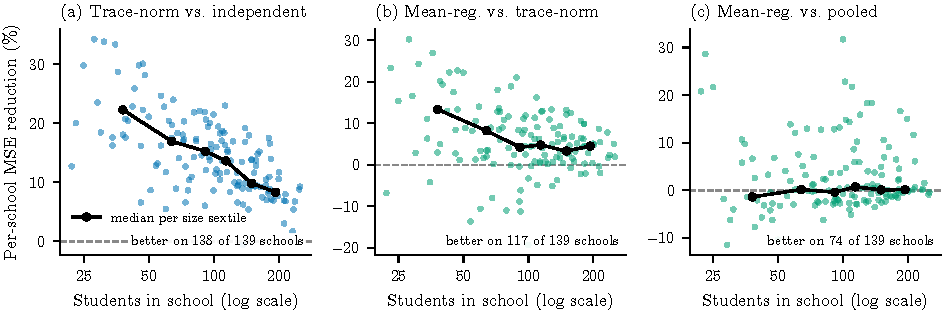
\includegraphics[width=\textwidth]{fig3_per_school.pdf}
\caption{Per-school change in test MSE at $\rho = 20\%$, averaged over 10 splits; positive values mean the first-named method is better. Each dot is one school, plotted against its size; the black line joins the median within six size groups. Sharing helps small schools most (a, b), while the gain of partial pooling over the pooled model is concentrated in a minority of schools of all sizes (c).}
\label{fig:per-school}
\end{figure}

\Cref{fig:per-school} breaks the gains down by school at $\rho = 20\%$. Trace-norm MTL improves on independent ridge for 138 of the 139 schools, and the improvement shrinks with school size (Spearman correlation $-0.63$): the median reduction in MSE is 17.6\% for schools below the median size and 10.4\% above it. Mean-regularized MTL improves on trace-norm MTL for 117 schools, again more for small schools (median 8.3\% against 4.5\%, Spearman $-0.27$, $p = 0.001$). Its 3.6\% advantage over the pooled model is distributed differently: it is better for only 74 of the 139 schools, with no relation to size (Spearman $0.10$, $p = 0.26$). The aggregate gain comes from a minority of schools that the pooled model fits poorly, several of which see reductions of 10 to 30\%.

\subsection{What structure is learned}
\label{sec:res-structure}

\begin{figure}[t]
\centering
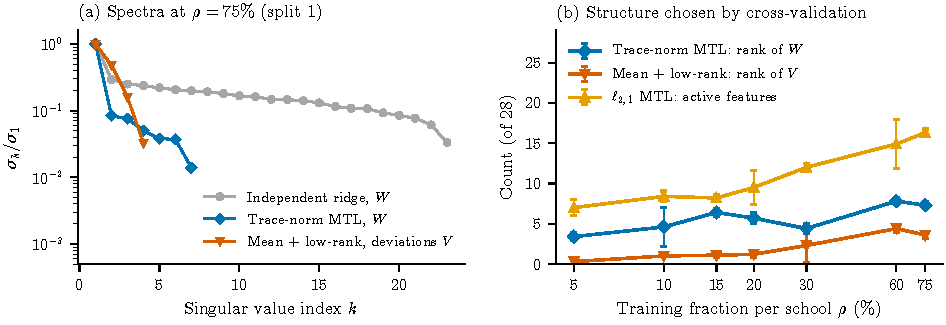
\includegraphics[width=\textwidth]{fig4_structure.pdf}
\caption{(a) Normalized singular values of the learned models at $\rho = 75\%$ (first split): the independent models, the trace-norm model and the deviations of the mean + low-rank model. (b) Structure selected by cross-validation as the training fraction grows: rank of the trace-norm model, rank of the mean + low-rank deviations and number of features kept by $\ell_{2,1}$ MTL (mean $\pm$ s.d.\ over 10 splits).}
\label{fig:structure}
\end{figure}

\Cref{fig:structure}a shows that the independent models do not share a low-dimensional subspace on their own: their singular values decay slowly ($\sigma_2/\sigma_1 = 0.29$) over a rank of 23. The trace-norm model concentrates almost all of its energy in one direction ($\sigma_2/\sigma_1 = 0.08$, rank 7), consistent with a dominant shared component. Once that component is modeled explicitly as a mean, the deviations need only a few directions (rank 4 in this split). \Cref{fig:structure}b shows that the selected structure grows with the data: $\ell_{2,1}$ MTL keeps 7 of 28 features at 5\% and 16 at 75\%, and the rank of the mean + low-rank deviations rises from below 1 on average at 5\% to about 4 at 60\% and 75\%. The rank of the trace-norm model changes less regularly, between 3 and 8, because the same directions must carry both the shared and the school-specific parts.

\subsection{Optimization: a fixed budget fails silently on unscaled features}
\label{sec:res-optim}

\begin{figure}[t]
\centering
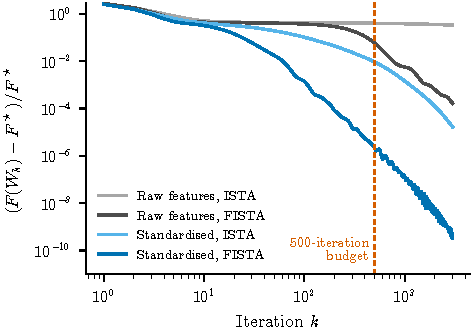
\includegraphics[width=0.56\textwidth]{fig5_optimisation.pdf}
\caption{Relative suboptimality of trace-norm MTL ($\lambda = 3$, $\rho = 75\%$, first split) for proximal gradient without (ISTA) and with (FISTA) momentum, on raw and standardized features. The dashed line marks the 500-iteration budget.}
\label{fig:optim}
\end{figure}

On raw features the two numeric columns take values up to 91 and 43, and the Lipschitz constant of the loss gradient is $L = 8{,}296$. Since the step size is $1/L$, progress per iteration is tiny: after 500 iterations FISTA is still 5.9\% above the optimal objective and ISTA 41\% above (\cref{fig:optim}). Standardizing the two columns lowers $L$ to 24.5, and FISTA then reaches a relative gap of $2.2 \times 10^{-6}$ within the same budget. Nothing in the output signals the difference, so fixed-budget solvers on unscaled data can produce unconverged models whose errors are then attributed to the method. All results in this paper use standardized features, and acceleration matters as well: on standardized features ISTA is still $9.4 \times 10^{-3}$ above the optimum after 500 iterations.

\subsection{Metric definitions change reported numbers}
\label{sec:res-metrics}

Explained variance on School is reported with two normalizations: by the variance of all test scores, or by the average variance within schools as in \eqref{eq:ev}. For identical predictions the two differ by 11.1 to 13.0 points (\cref{tab:metrics}): trace-norm MTL scores 26.5\% under the within-school definition and 37.9\% under the pooled one. The pooled definition credits a model for explaining differences between schools, which make up 11.5\% of the variance. Rankings are unchanged, but absolute values are not comparable across papers that normalize differently, and published numbers should be compared only after the definition is confirmed.
